%!TEX root = ../Thesis.tex

\chapter{Clusteranalyse von Fahrzeugtrajektorien}
\label{cha:realisation_clustering}

In diesem Kapitel wird die Umsetzung der Clusteranalyse der Trajektorien vorgestellt.
Es wird zuerst darauf eingegangen, welche Trajektorie-Repräsentation gewählt wurde. Anschließend
werden die verschiedenen Schritte zur Bereinigung und Vorverarbeitung der Daten beschrieben, welche
in dieser Arbeit zum Einsatz kommen. Schlussendlich folgt die Erläuterung der eigentlichen Clusteranalyse.
Hier werden die verschiedenen untersuchten Ansätze vorgestellt und ihre Ergebnisse diskutiert.

Die \textit{TrackerApplication} ist in Java und Scala implementiert. Ihre Benutzeroberfläche basiert
auf JavaFX. Das in dieser Arbeit erstellte Modul \textit{Spurerkennung} wird komplett mit Scala umgesetzt. 

\section{Erstellen von Trajektorien}

Die Ergebnisse der Fahrzeugverfolgung (siehe Abschnitt \ref{sec:position_extraction}) werden
in der \textit{TrackingApplication} in Form sogenannter \textit{TrackedObject}`s gespeichert.
Ein solches Objekt repräsentiert eine zusammenhängende, nicht-unterbrochene Verfolgung eines Fahrzeugs.
Die wichtigsten Informationen, die ein \textit{TrackedObject} beinhaltet, sind eine eindeutige ID,
die Frame-Positionen des Starts und Endes der Verfolgung und die Objekt-Klasse des Fahrzeugs. Es wird
zwischen den vier Klassen \textit{``Auto''}, \textit{``Lastwagen''}, \textit{``Transporter''}
und \textit{``Zweirad''} unterschieden.
Für jedes verfolgte Objekt können die zugehörigen Positions-, Geschwindigkeits-, Beschleunigungs-
und Dimensions-Informationen abgerufen werden. Diese werden für jedes Frame, welches zwischen dem Start-
und End-Frame des Objektes liegt, bestimmt.

Da für die Ableitung von Fahrspuren aus Trajektorien lediglich die positionsbezogenen Eigenschaften
der Fahrzeuge relevant sind, werden Bewegungbahnen in dieser Arbeit über jene definiert.
Geschwindigkeit, Beschleunigung und Dimension der Fahrzeuge wird in der Clusteranalyse nicht berücksichtigt.
Abbildung \ref{fig:real_trajectory_classDia} zeigt den Aufbau einer Trajektorie im Modul \textit{Spurerkennung}.

\begin{figure}[H]
\centering
    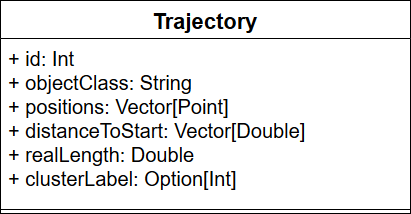
\includegraphics[width=0.38\linewidth]{../resources/img/umsetzung/U1/Trajectory_ClassDia}
\caption{Aufbau Trajektorie-Klasse}
\label{fig:real_trajectory_classDia}
\end{figure}

Die Felder \textit{id} und \textit{objectClass} werden aus dem der Trajektorie zugrundeliegenden \textit{TrackedObject}
übernommen. 
Die Positionen eines Fahrzeugs werden in Form von 2D-Welt-Koordinaten (siehe Abschnitt \ref{sec:position_extraction})
in \textit{positions} gespeichert.
Die Sequenz \textit{distToStart} enthält für jeden Punkt der Bewegungsbahn die Distanz zum Start der Trajektorie in Metern.
Die Werte ergeben sich aus Formel \ref{eq_real_distToStart}, wobei $p_n$ dem $n$-ten Punkt in der Trajektorie entspricht
und $dist$ der euklidschen Distanz zwischen zwei Punkten.

\begin{ceqn}
\begin{align}
\label{eq_real_distToStart}
    distToStart(p_n) =
    \begin{cases}
        0 & \text{if } n = 0 \\
        dist(p_n,\ p_{n-1}) + distToStart(p_{n-1}) & \text{otherwise} 
    \end{cases}
\end{align}
\end{ceqn}

Aus \textit{distToStart} ergibt sich zudem die Gesamtlänge einer Trajektorie, welche extra gespeichert wird.
Das Feld \textit{clusterLabel} ordnet jede Trajektorie nach der Clusteranalyse einem bestimmten Cluster zu.
Zuvor enthält es keinen Wert.

% TODO: Evtl Bilder und Beschreibung austauschen
Zur Untersuchung der Fahrzeugtrajektorien ist es hilfreich diese zu visualisieren. Abbildung \ref{fig:real_trajs_raw_neckartor}
zeigt so beispielsweise 1240 Trajektorien, welche aus einer Aufnahme des Stuttgarter Neckartors extrahiert wurden.
In Abbildung \ref{fig:real_neckartor} ist ein Ausschnitt der entsprechenden Aufnahme zu sehen.

\begin{figure}[H]
\centering
    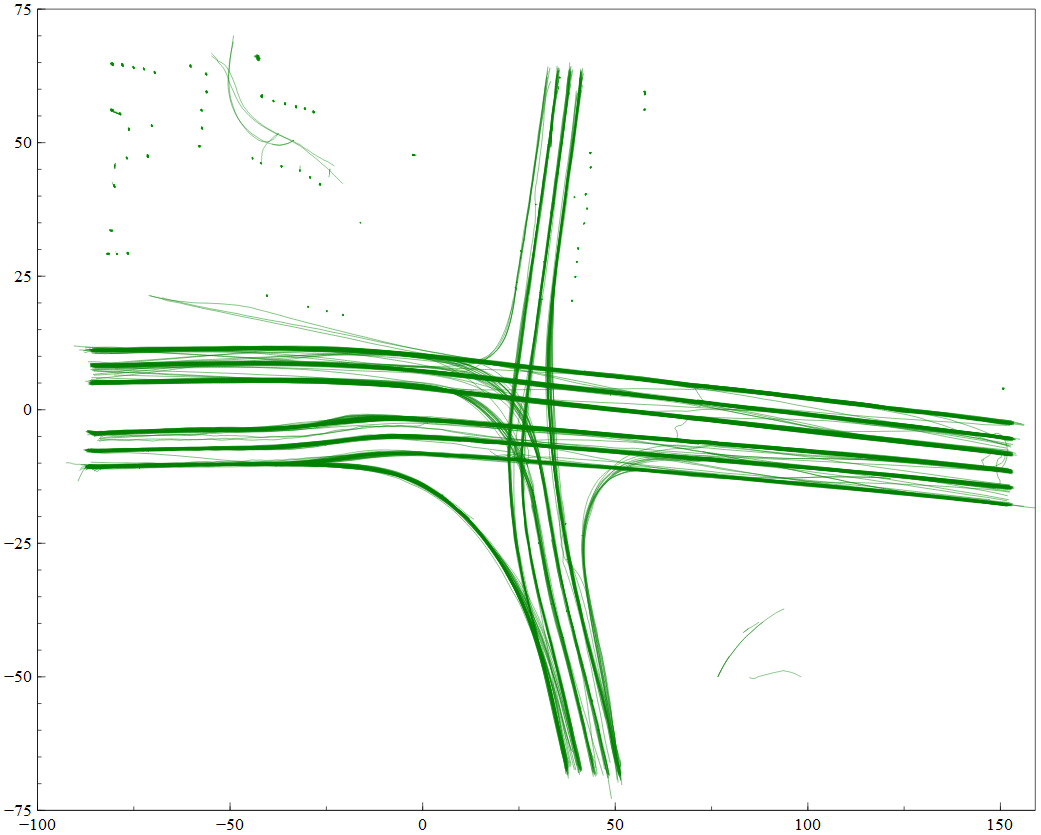
\includegraphics[width=0.55\linewidth]{../resources/img/umsetzung/U1/Plot_RawTrajectories_Neckartor}
\caption{Unverarbeitete Trajektorien vom Stuttgarter Neckartor}
\label{fig:real_trajs_raw_neckartor}
\end{figure}

\begin{figure}[H]
\centering
    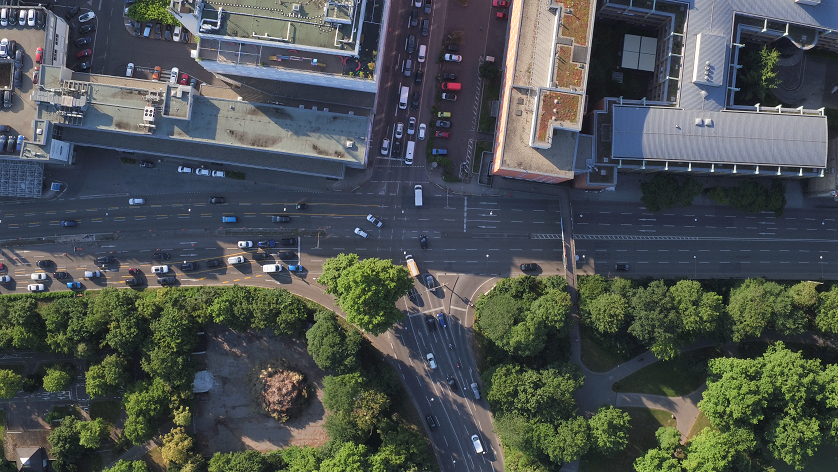
\includegraphics[width=0.8\linewidth]{../resources/img/umsetzung/U1/Neckartor_Aufnahme}
\caption{Das Stuttgarter Neckartor}
\label{fig:real_neckartor}
\end{figure}

In Abbildung \ref{fig:real_trajs_raw_neckartor} sind die verschiedenen Bewegungsbahnen der Fahrzeuge für
den menschlichen Betrachter bereits klar erkennbar.
Direkt fallen aber auch die Trajektorien der stehenden oder sich auf Parkplätzen
bewegenden Autos im oberen Bereich der Aufnahme ins Auge. Diese dürfen nicht in die Clusteranalyse mit einbezogen werden.
Bei genauerer Untersuchung der Trajektorien zeigen sich weitere Probleme, welche das Clustering negativ
beeinflussen würden. Zwei sind in nachfolgender Abbildung dargestellt.
\ref{fig:real_defects_trajectories} a) zeigt, wie Fahrzeuge Punktwolken beim Stilstand vor Lichtsignalanlagen bilden.
In \ref{fig:real_defects_trajectories} b) wird deutlich, dass in manchen Bereichen sehr viele Trajektorie-Unterbrechungen
auftreten. Hier wird die Straße üblicherweise von Bäumen, Brücken et cetera überlagert.

\begin{figure}[H]
    \centering
    \subfloat[]{{
        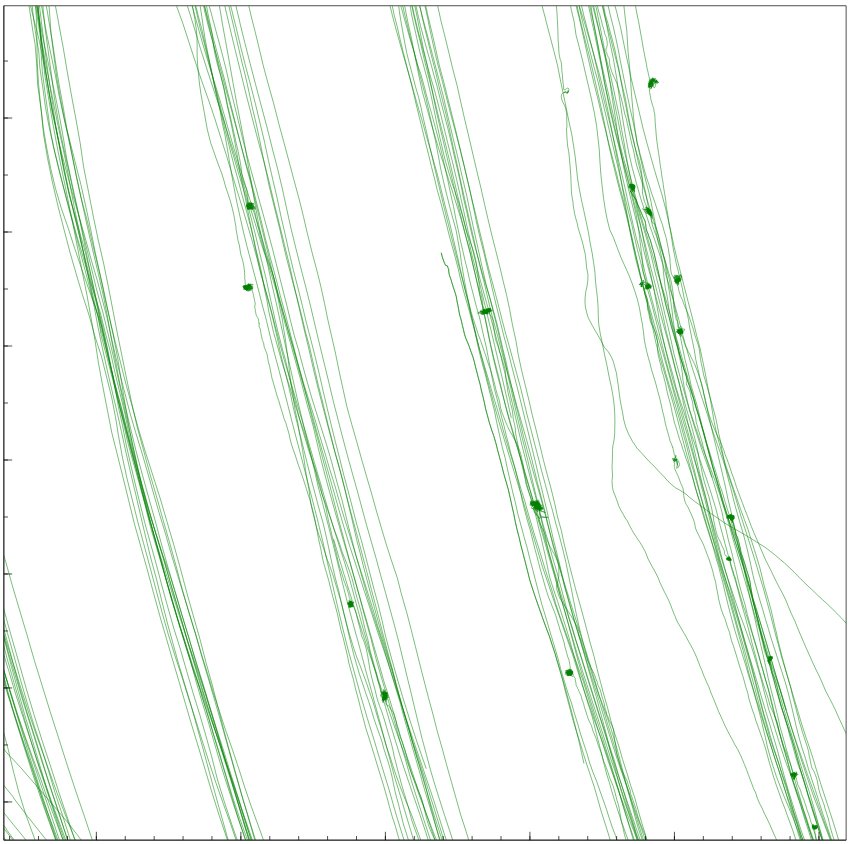
\includegraphics[align=c, width=0.4\linewidth]{../resources/img/umsetzung/U1/trajectories_defect1}
    }}
    \subfloat[]{{
        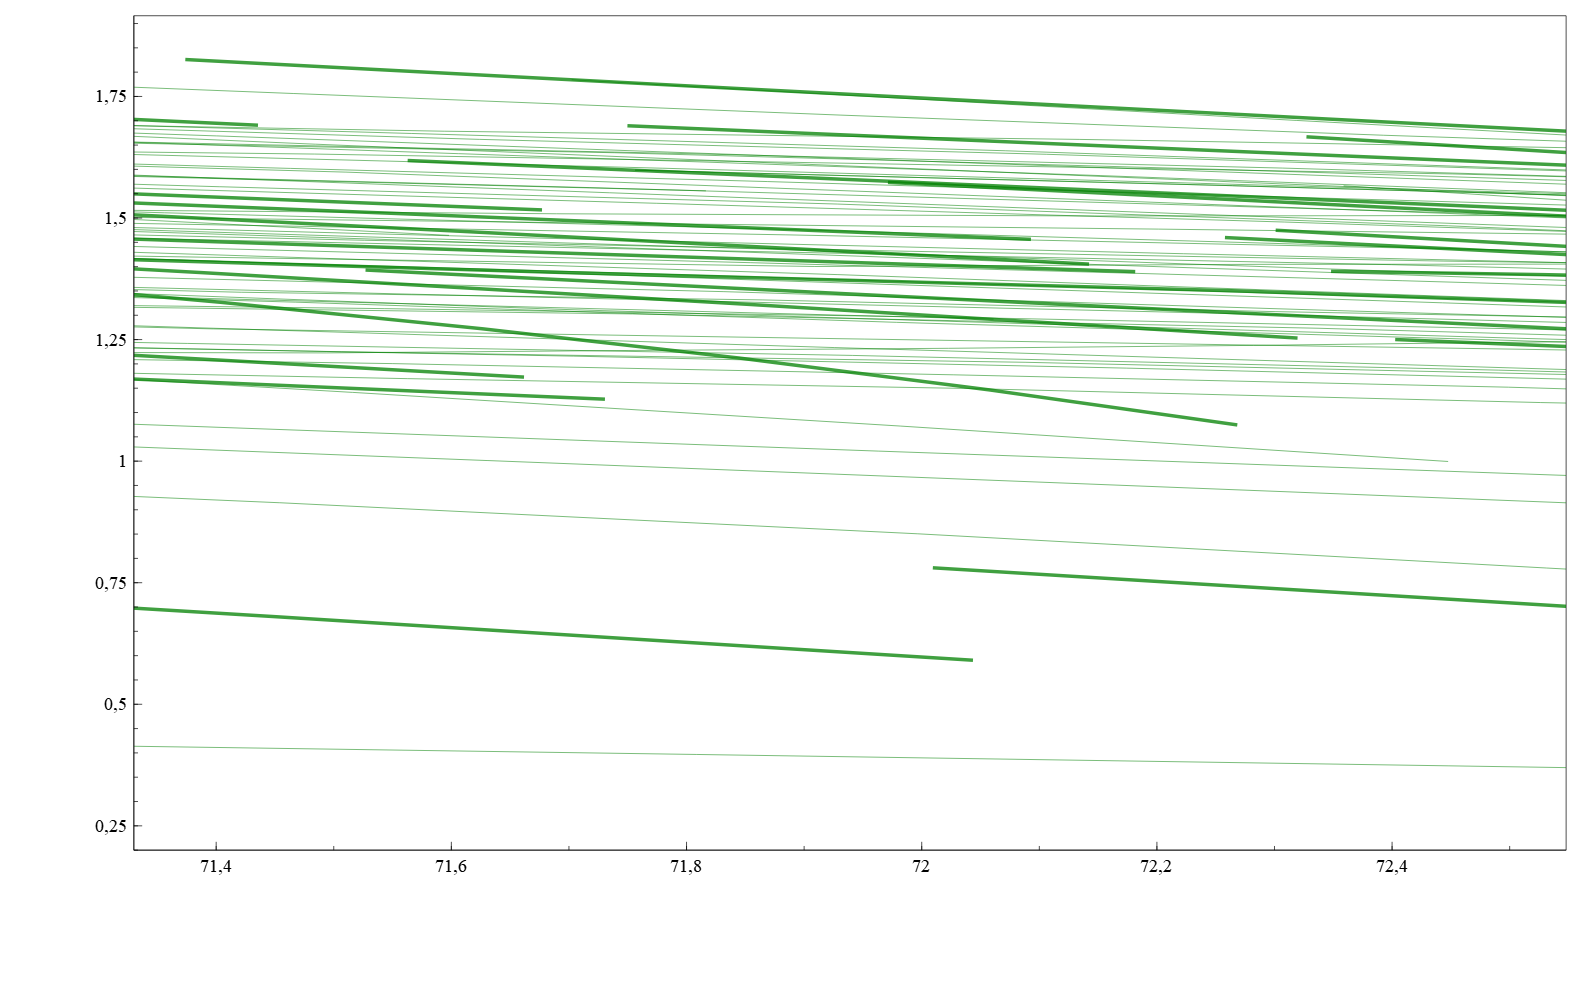
\includegraphics[align=c, width=0.5\linewidth]{../resources/img/umsetzung/U1/trajectories_defect2}
    }}
    \caption{a) Punktwolken vor Lichtsignalanlagen, b) Unterbrechungen aufgrund von Überdeckung}
    \label{fig:real_defects_trajectories}
\end{figure}

Um von diesen und weiteren Effekten bei der Clusteranalyse nicht beeinflusst zu werden, durchlaufen die
``Roh-Trajektorien'' einen Vorverarbeitungsschritt. Dieser wird im nächsten Abschnitt vorgestellt.

\section{Vorverarbeitung der Trajektorien}
\label{sec:realisation_preprocessing}

% Aussortierung zu kurzer Trajektorien
%   Stehend, Teiltrajectorien etc.
% Resampling (wichtig Datenmenge)
% Aussortierung zu kurzer Trajektorien
% Prüfen isCompleteTraj.
%   Unterbrochene Traj. ausfiltern
% Trimmen Truck-Trajektories

% Wird eine Fahrzeugverfolgung, beispielsweise aufgrund von Überdeckungen, unterbrochen, so wird ein
% Kraftfahrzeug von mehreren \textit{TrackedObjects} repräsentiert, welche sich allerdings nicht einander
% zuordnen lassen.

\section{Clustering der Trajektorien}
\label{sec:realisation_clustering}

% genaue Beschreibung des Vorgehens, bis finale Clustering Lösung erreicht wurde
% Ansätze: Gründe, Stärken, tatsächliche Problem
% Ansatz A:
%   Mod. Hausdorff Distanz und Spectral Clustering (bas. auf Avet et al.) (Erklärung Grundfunktionsweise Spectral-Clustering)
%   Weil: SC performant, deterministisch, oft verwendet
%   Probleme: Clusteranzahl Bestimmung, Umgehen mit Ausreißern, Tatsächliche Ergebnisse nicht gut
%   --> Performance / Qualität des Ansatzes konnte für vorhandene Daten nicht bestätigt werden
%   --> Problematisch auch Umgang mit vielen Parametern
% Ansatz B:
%   LCSS Distanz (in anderen Papern gute Ergebnisse) (impl. mittels bottom up dyna. programmierung, Verwendung Eucl. Dist.)
%   Wieso D2 aus Vlachos et al. verwendet? (Verschiebung unerwünscht)
%   DBSCAN Clustering
%   --> DM kann besser mit Ausreißern umgehen und DBSCAN berücksichtigt diese auch
%   bessere Ergebnisse

% Probleme: Erkennung von Abbiegespuren, mit wenig Fahrzeugen und Abbiegevorgängen auf mehrere Spuren
%   Dafür: Weitere Verarbeitung der Clustering Outlier
%   Beschreibung Verfahren (dichte-basiert, suchen von initial Dichten Regionen, Verfolgung bis Ausdünnung)

\chapter{Fahrspur-Bestimmung aus Trajektorie-Clustern}
\label{cha:lane_definition}

% Cluster-Bereinigung: Entfernen von Outliern (Spurwechselvorgänge)
%   Beschreibung Probleme: Performance, Zuverlässigkeit (initial Distanzbasiert, erweitert Dichtebasiert --> Ähnliche Ergebnisse und Performance)
%   Verfahren mit evtl. besseren Resultaten noch aufwendiger und basierend meist auf selben Ideen (Distanzmaße, Dichten etc.)
% Bestimmung Referenz-Trajektorie
% Bestimmung von Spur-Envelopes
% Partitionierung der initialen Spur-Schätzungen
% Alignment der Spuren